\section{Introduction}
\subsection{Nuclear Energy}
\frame
{
  \frametitle{Nuclear Energy Perspective}
	\begin{itemize}
		\item<1-> Nuclear energy provides about 10\% of the world's electricity from about 450 power reactors.
		\item<2-> Nuclear is the world's second largest source of low-carbon power (29\% of the total in 2017).
			\begin{figure}[htbp]
			\begin{center}
			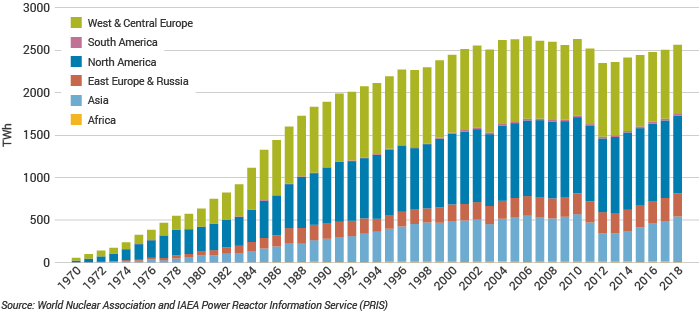
\includegraphics[width=0.75\textwidth]{Figures/Nuclear_2019}
			\end{center}
			\end{figure}
		\item<3-> Nuclear power capacity worldwide is increasing steadily, with about 50 reactors under construction.
	\end{itemize}
}

\frame{
	\frametitle{Nuclear Reactors}
	\begin{itemize}
		\item<1-> Nuclear reactors are used to carry out controlled chain reactions to produce heat through fission.
		\item<2-> Most of the reactors currently in use are 2\textsuperscript{nd} / 3\textsuperscript{rd}  generation Light Water Reactors or Pressurised Heavy Water Reactors.
			\begin{figure}[htbp]
			\begin{center}
				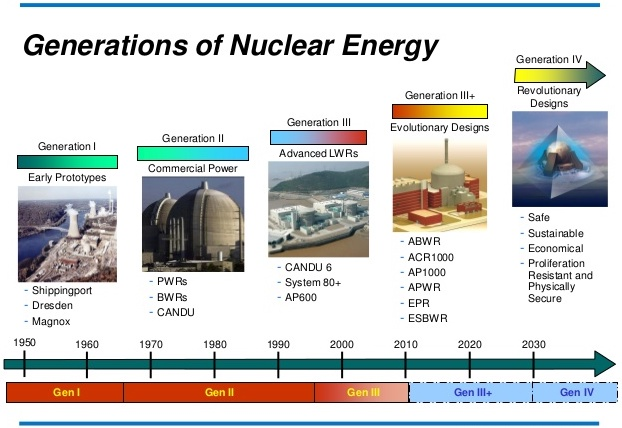
\includegraphics[height=0.5\paperheight]{Figures/Gen_Nuclear}	
			\end{center}
			\end{figure}
	\end{itemize}
}

\frame{
	\frametitle{Simulation of Nuclear Reactors}
	\begin{itemize}
		\item Traditional reactor simulation tools rely on the \emph{Operator Splitting} approach.
	\end{itemize}
	\pause	
	\begin{figure}[htbp]
		\begin{center}
			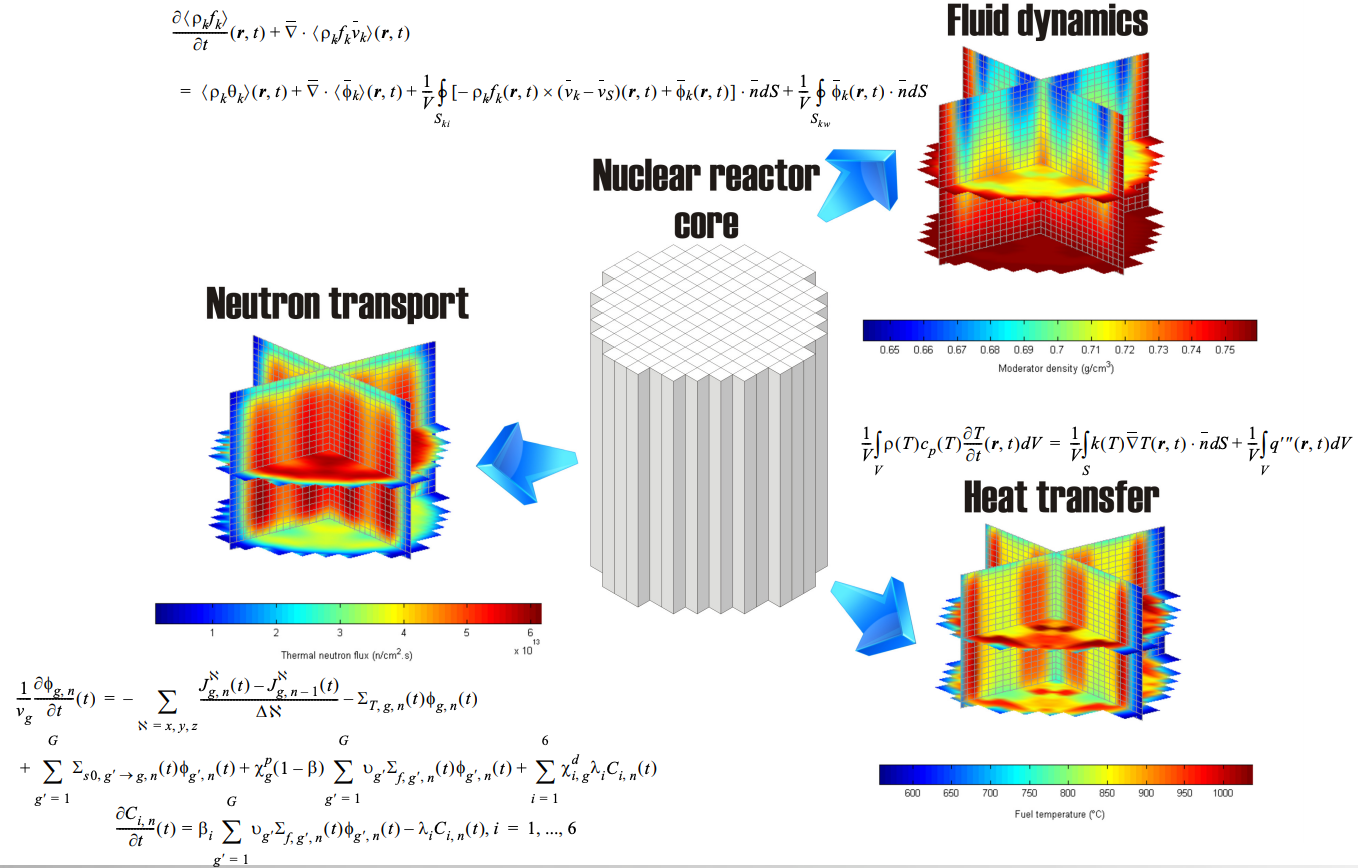
\includegraphics[height=0.55\paperheight]{Figures/Operator_split}	
		\end{center}
	\end{figure}
}

\subsection{Generation IV Reactors}
\frame{
	\frametitle{Generation IV Reactors}
	\only<1-5>{\begin{itemize}
		\item<1-> Generation IV reactors are advanced reactor concepts under development with the following goals:
			\begin{itemize}
				\item <2-> Sustainability
				\item <3-> Economy
				\item <4-> Safety and reliability
				\item <5-> Proliferation resistance
			\end{itemize}
	\end{itemize}}	
	\only<6>{\begin{figure}[htbp]
		\begin{center}
			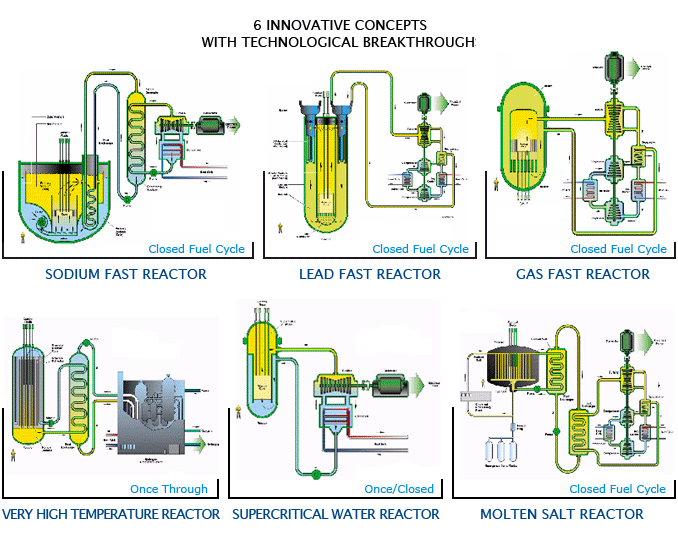
\includegraphics[width=0.75\paperwidth,height=0.75\paperheight]{Figures/gen_4_concepts}	
		\end{center}
	\end{figure}}
}

\frame{
	\frametitle{Molten Salt Reactor}
	\only<1-2>{\begin{itemize}
		\item Molten Salt Reactor (MSR) are the reference circulating fuel concept under the Generation IV framework.
	\end{itemize}}	
	\only<2>{\begin{figure}[htbp]
		\begin{center}
			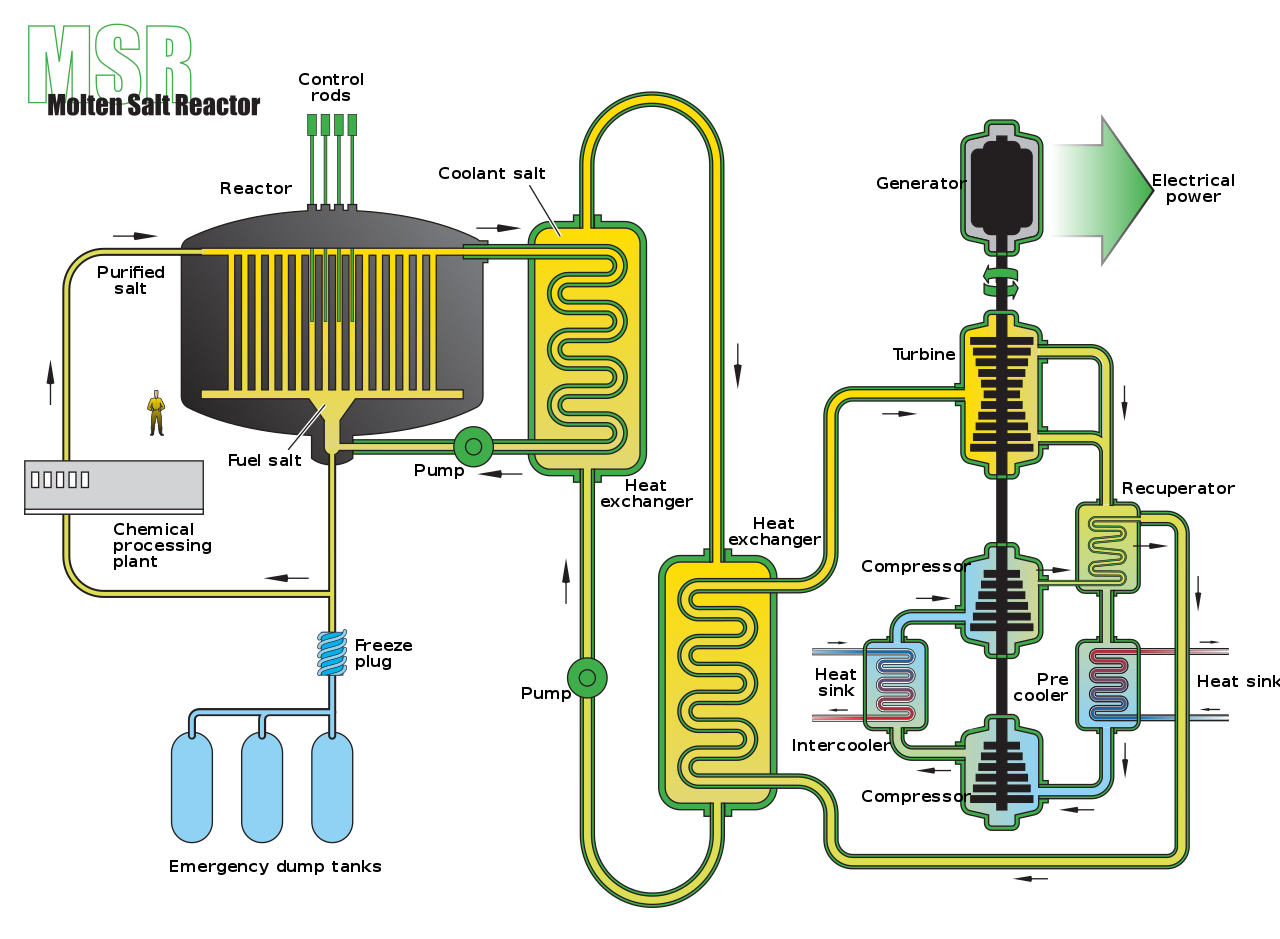
\includegraphics[height=0.65\paperheight]{Figures/MSR}	
		\end{center}
	\end{figure}}
	\only<3-4> 
	{\begin{itemize}
		\item MSR exhibit very tight coupling between different physical phenomena.
	\end{itemize}}	
	\only<4>{\begin{figure}[htbp]
		\begin{center}
			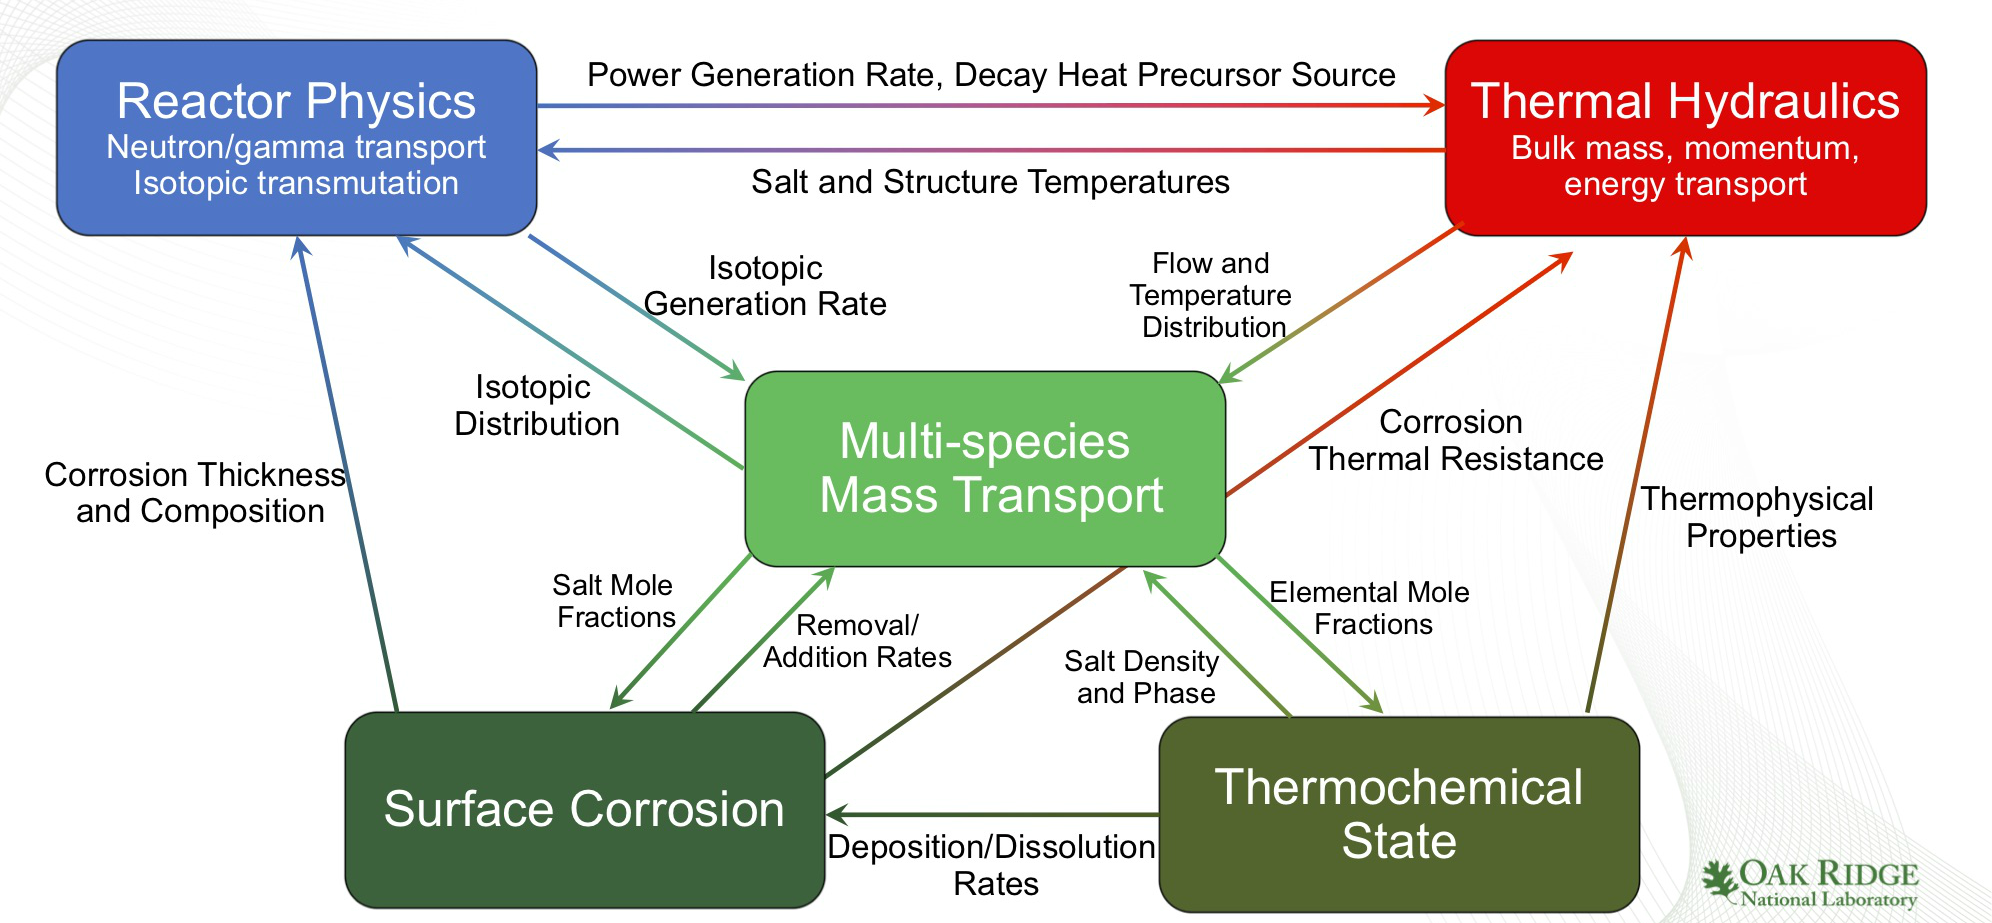
\includegraphics[height=0.55\paperheight]{Figures/MSR_MPH}	
		\end{center}
	\end{figure}}
}

\subsection{Multiphysics Simulations}
\frame{
	\frametitle{MOOSE}
	\only<1-5>{\begin{itemize}
		\item<1-> Design and simulation of advanced reactors requires advanced multiphysics tools.
		\item<2-> Multiphysics Object Oriented Simulation Environment (MOOSE) is a finite element framework for solving computational engineering problems.
		\item<3-> Developed by the Idaho National Laboratory and open-source since 2014.
		\item<4-> MOOSE follows a Nuclear Quality Assurance Level 1 (NQA-1) development process.
		\item<5-> MOOSE includes a test suite and documentation system to allow for agile development while maintaining a NQA-1 process.
	\end{itemize}}
	\only<6>{\begin{figure}[htbp]
		\begin{center}
			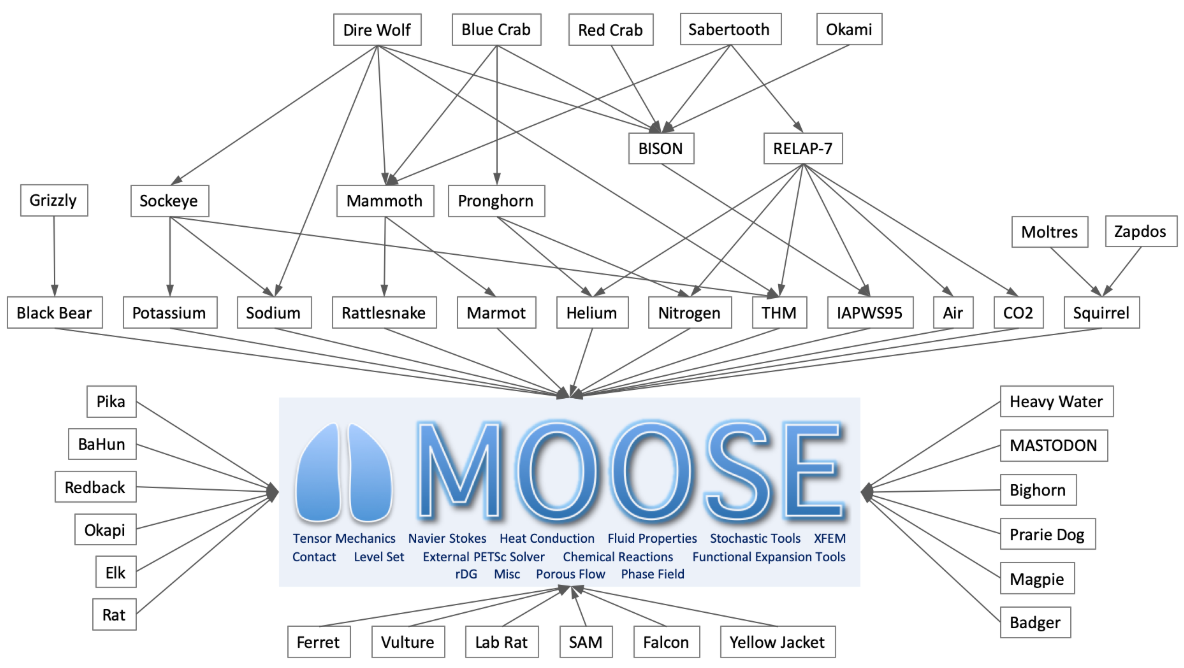
\includegraphics[width=0.85\paperwidth]{Figures/moose}	
		\end{center}
	\end{figure}}
}


\frame{
	\frametitle{Nuclear Materials}
	\only<1-2>{\begin{itemize}
		\item<1-> Nuclear materials are highly complex multiscale, multiphysics systems.
	\end{itemize}}
	\only<2>{\begin{figure}[htbp]
		\begin{center}
			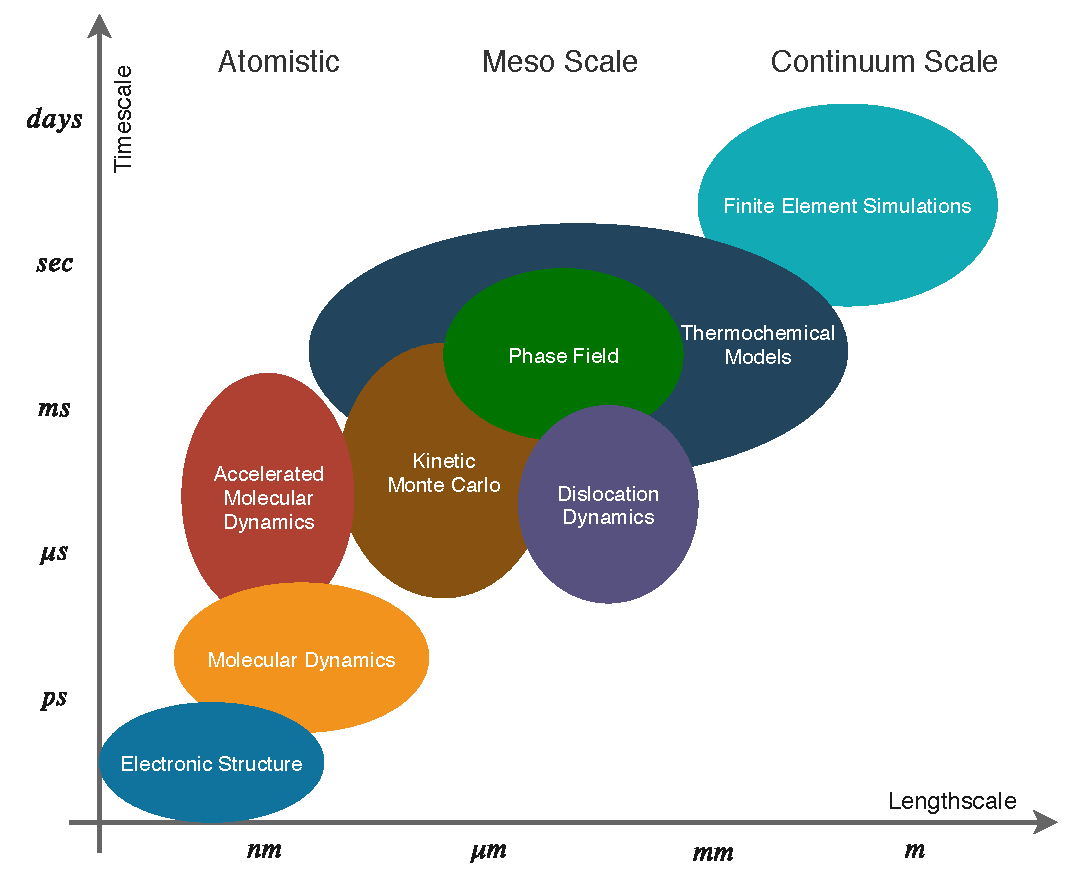
\includegraphics[height=0.5\paperheight]{Figures/Multiphysics.pdf}	
		\end{center}
	\end{figure}}
	\only<3>{\begin{figure}[htbp]
		\begin{center}
			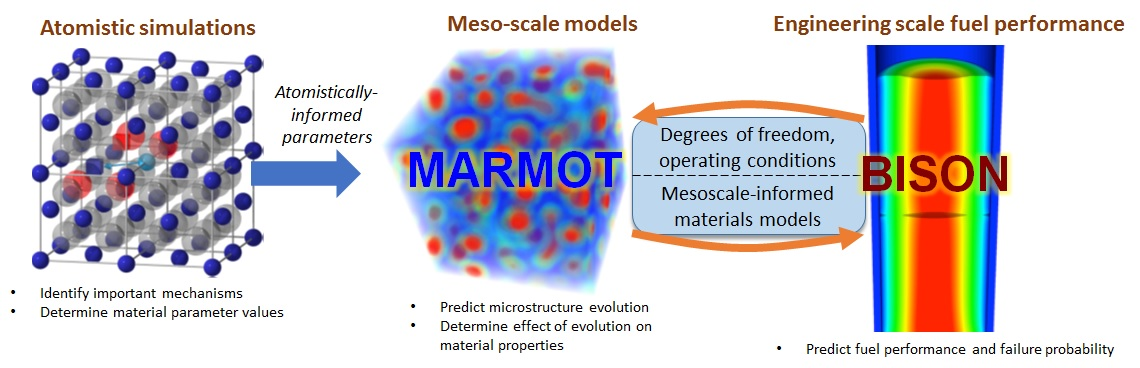
\includegraphics[width=0.85\paperwidth]{Figures/FPL}	
		\end{center}
		\end{figure}}
}

\frame{
	\frametitle{Corrosion}
	\begin{itemize}
		\item<1-> MSR and other advanced reactors use high temperature fluids such as molten fluoride/chloride salts.
		\item<2-> High temperature fluids especially molten fluoride/chloride salts cause corrosion of  structural materials.
		\item<3-> Corrosion is an electrochemical process driven by the thermodynamic and kinetics of the system.
		\item<4-> Effective prediction of corrosion requires a multiscale, mutiphysics approach.
	\end{itemize}
	\onslide<5->
	{\begin{alertblock}{}
		\centering {Currently, MOOSE lacks a corrosion modelling tool!}
	\end{alertblock}}
}

\frame{
	\frametitle{Yellowjacket}
	\only<1-3>{\begin{itemize}
		\item<1-> Yellowjacket is a new corrosion modelling tool currently under development.
		\item<2-> Yellowjacket will couple phase field models with thermodynamic equilibrium calculations to  effectively model corrosion in advanced reactors.
		\item<3-> Collaboration between Ontario Tech University, University of Florida, Idaho National Laboratory and Los Alamos National Laboratory.
	\end{itemize}}
	\only<4->{\begin{figure}[htbp]
		\begin{center}
			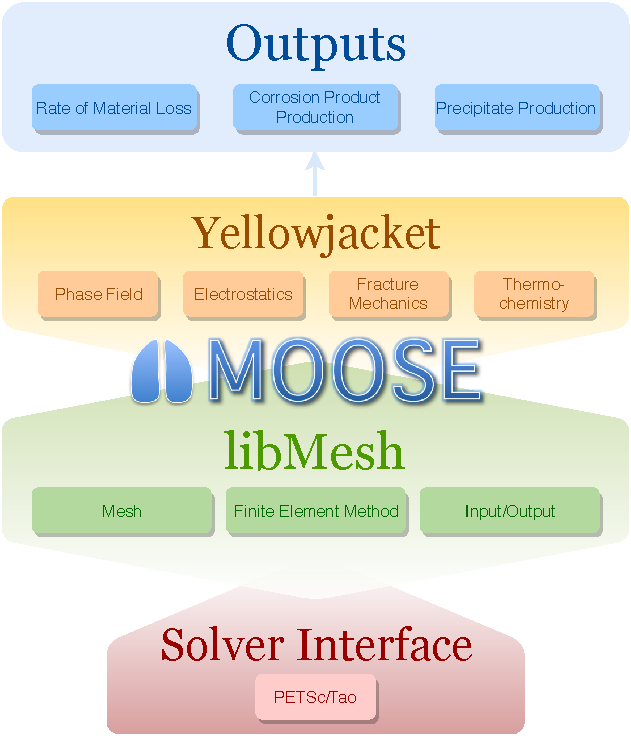
\includegraphics[height=0.75\paperheight]{Figures/Yellowjacket_MOOSE.pdf}	
		\end{center}
		\end{figure}
	}
}

\frame{
	\frametitle{Thermodynamics in Yellowjacket}
	\only<1-4>{\begin{itemize}
		\item<1-> Phase and chemical behaviour of nuclear materials is governed by the thermodynamic equilibrium state.
		\item<2-> The composition of nuclear materials continuously evolves under irradiation affecting the equilibrium state.
		\item<3-> Capturing thermodynamic equilibria has traditionally relied on empirical correlations.
		\item<4-> Direct coupling of thermodynamic equilibrium can augment multiphysics calculations by providing quantities such as the chemical potentials, Gibbs energies, etc. 
	\end{itemize}}
	\only<5->{\begin{figure}[htbp]
		\begin{center}
			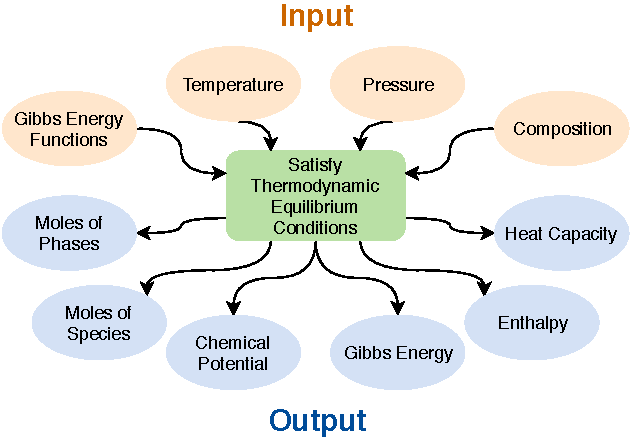
\includegraphics[height=0.5\paperheight]{Figures/Thermodynamics.pdf}	
		\end{center}
		\end{figure}
	}
}




























